

\tikzset{every picture/.style={line width=0.75pt}} %set default line width to 0.75pt        

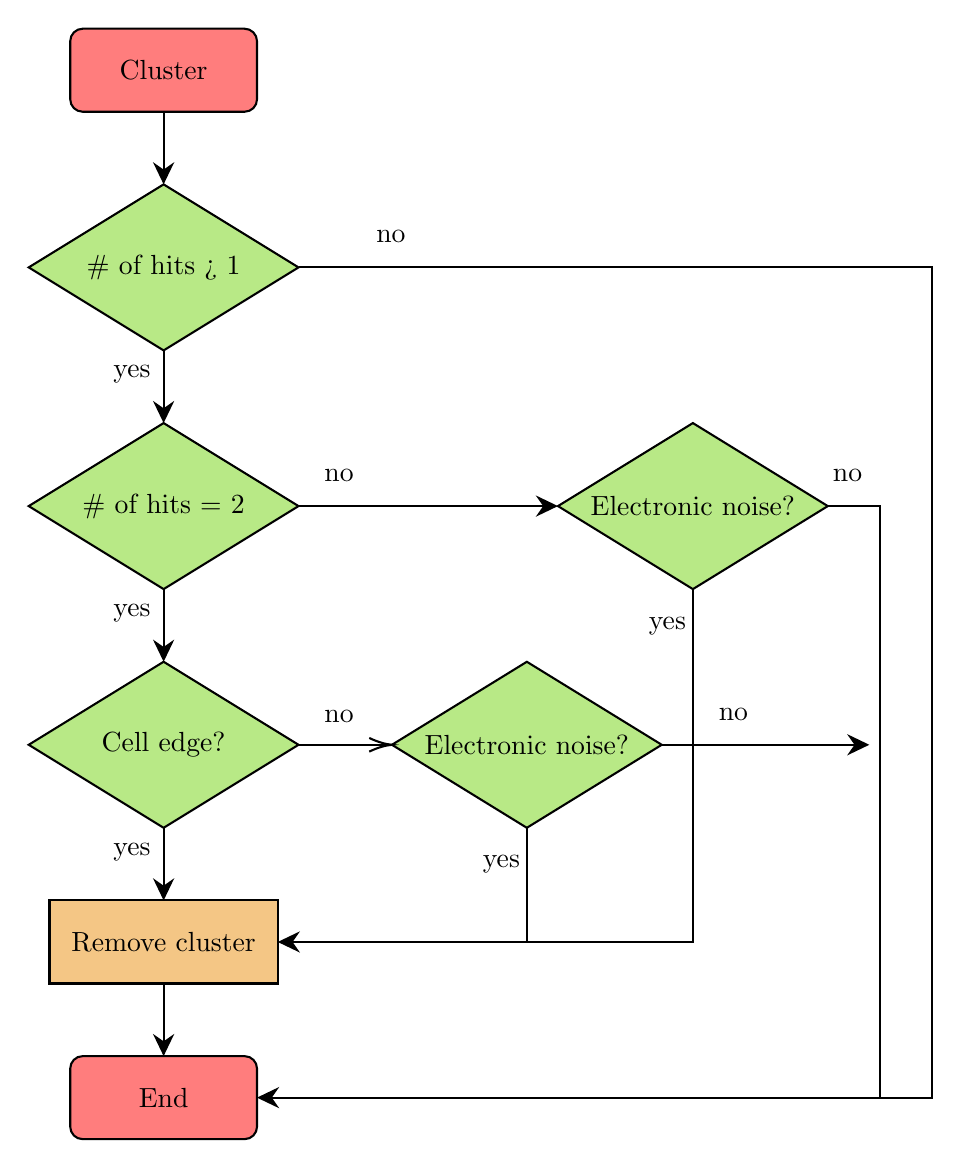
\begin{tikzpicture}[x=0.75pt,y=0.75pt,yscale=-1,xscale=1]
	%uncomment if require: \path (0,782); %set diagram left start at 0, and has height of 782

	%Rounded Rect [id:dp1662492856064861] 
	\draw  [fill={rgb, 255:red, 255; green, 125; blue, 125 }  ,fill opacity=1 ] (20,11) .. controls (20,7.69) and (22.69,5) .. (26,5) -- (104,5) .. controls (107.31,5) and (110,7.69) .. (110,11) -- (110,39) .. controls (110,42.31) and (107.31,45) .. (104,45) -- (26,45) .. controls (22.69,45) and (20,42.31) .. (20,39) -- cycle ;
	%Flowchart: Decision [id:dp816640900376574] 
	\draw  [fill={rgb, 255:red, 184; green, 233; blue, 134 }  ,fill opacity=1 ] (240,310) -- (305,350) -- (240,390) -- (175,350) -- cycle ;
	%Flowchart: Decision [id:dp3056798665151721] 
	\draw  [fill={rgb, 255:red, 184; green, 233; blue, 134 }  ,fill opacity=1 ] (320,195) -- (385,235) -- (320,275) -- (255,235) -- cycle ;
	%Straight Lines [id:da43332826362990795] 
	\draw    (65,45) -- (65,77) ;
	\draw [shift={(65,80)}, rotate = 270] [fill={rgb, 255:red, 0; green, 0; blue, 0 }  ][line width=0.08]  [draw opacity=0] (10.72,-5.15) -- (0,0) -- (10.72,5.15) -- (7.12,0) -- cycle    ;
	%Straight Lines [id:da1721933893310973] 
	\draw    (65,160) -- (65,192) ;
	\draw [shift={(65,195)}, rotate = 270] [fill={rgb, 255:red, 0; green, 0; blue, 0 }  ][line width=0.08]  [draw opacity=0] (10.72,-5.15) -- (0,0) -- (10.72,5.15) -- (7.12,0) -- cycle    ;
	%Straight Lines [id:da7629068372469668] 
	\draw    (130,235) -- (252,235) ;
	\draw [shift={(255,235)}, rotate = 180] [fill={rgb, 255:red, 0; green, 0; blue, 0 }  ][line width=0.08]  [draw opacity=0] (10.72,-5.15) -- (0,0) -- (10.72,5.15) -- (7.12,0) -- cycle    ;
	%Straight Lines [id:da2682927683523839] 
	\draw    (130,350) -- (173,350) ;
	\draw [shift={(175,350)}, rotate = 180] [color={rgb, 255:red, 0; green, 0; blue, 0 }  ][line width=0.75]    (10.93,-3.29) .. controls (6.95,-1.4) and (3.31,-0.3) .. (0,0) .. controls (3.31,0.3) and (6.95,1.4) .. (10.93,3.29)   ;
	%Shape: Rectangle [id:dp937184065620104] 
	\draw  [fill={rgb, 255:red, 244; green, 198; blue, 133 }  ,fill opacity=1 ] (10,425) -- (120,425) -- (120,465) -- (10,465) -- cycle ;
	%Straight Lines [id:da7703418793683412] 
	\draw    (130,120) -- (435,120) -- (435,520) -- (113,520) ;
	\draw [shift={(110,520)}, rotate = 360] [fill={rgb, 255:red, 0; green, 0; blue, 0 }  ][line width=0.08]  [draw opacity=0] (10.72,-5.15) -- (0,0) -- (10.72,5.15) -- (7.12,0) -- cycle    ;
	%Straight Lines [id:da9159913508501855] 
	\draw    (385,235) -- (410,235) -- (410,520) ;
	%Straight Lines [id:da9876271822829807] 
	\draw    (305,350) -- (402,350) ;
	\draw [shift={(405,350)}, rotate = 180] [fill={rgb, 255:red, 0; green, 0; blue, 0 }  ][line width=0.08]  [draw opacity=0] (10.72,-5.15) -- (0,0) -- (10.72,5.15) -- (7.12,0) -- cycle    ;
	%Straight Lines [id:da06393806538831526] 
	\draw    (320,275) -- (320,445) -- (123,445) ;
	\draw [shift={(120,445)}, rotate = 360] [fill={rgb, 255:red, 0; green, 0; blue, 0 }  ][line width=0.08]  [draw opacity=0] (10.72,-5.15) -- (0,0) -- (10.72,5.15) -- (7.12,0) -- cycle    ;
	%Straight Lines [id:da5394607907564043] 
	\draw    (240,390) -- (240,445) ;
	%Rounded Rect [id:dp009664062523304096] 
	\draw  [fill={rgb, 255:red, 255; green, 125; blue, 125 }  ,fill opacity=1 ] (20,506) .. controls (20,502.69) and (22.69,500) .. (26,500) -- (104,500) .. controls (107.31,500) and (110,502.69) .. (110,506) -- (110,534) .. controls (110,537.31) and (107.31,540) .. (104,540) -- (26,540) .. controls (22.69,540) and (20,537.31) .. (20,534) -- cycle ;
	%Flowchart: Decision [id:dp9024602763737721] 
	\draw  [fill={rgb, 255:red, 184; green, 233; blue, 134 }  ,fill opacity=1 ] (65,80) -- (130,120) -- (65,160) -- (0,120) -- cycle ;
	%Flowchart: Decision [id:dp13524885014891452] 
	\draw  [fill={rgb, 255:red, 184; green, 233; blue, 134 }  ,fill opacity=1 ] (65,195) -- (130,235) -- (65,275) -- (0,235) -- cycle ;
	%Flowchart: Decision [id:dp2973369440123841] 
	\draw  [fill={rgb, 255:red, 184; green, 233; blue, 134 }  ,fill opacity=1 ] (65,310) -- (130,350) -- (65,390) -- (0,350) -- cycle ;
	%Straight Lines [id:da3005280685773618] 
	\draw    (65,275) -- (65,307) ;
	\draw [shift={(65,310)}, rotate = 270] [fill={rgb, 255:red, 0; green, 0; blue, 0 }  ][line width=0.08]  [draw opacity=0] (10.72,-5.15) -- (0,0) -- (10.72,5.15) -- (7.12,0) -- cycle    ;
	%Straight Lines [id:da23847540301482073] 
	\draw    (65,390) -- (65,422) ;
	\draw [shift={(65,425)}, rotate = 270] [fill={rgb, 255:red, 0; green, 0; blue, 0 }  ][line width=0.08]  [draw opacity=0] (10.72,-5.15) -- (0,0) -- (10.72,5.15) -- (7.12,0) -- cycle    ;
	%Straight Lines [id:da3670573044208534] 
	\draw    (65,465) -- (65,497) ;
	\draw [shift={(65,500)}, rotate = 270] [fill={rgb, 255:red, 0; green, 0; blue, 0 }  ][line width=0.08]  [draw opacity=0] (10.72,-5.15) -- (0,0) -- (10.72,5.15) -- (7.12,0) -- cycle    ;

	% Text Node
	\draw (65,25) node   [align=left] {\begin{minipage}[lt]{34.68pt}\setlength\topsep{0pt}
			\begin{center}
				Cluster
			\end{center}

		\end{minipage}};
	% Text Node
	\draw (65,120) node   [align=left] {\begin{minipage}[lt]{60pt}\setlength\topsep{0pt}
			\begin{center}
				\# of hits > 1
			\end{center}

		\end{minipage}};
	% Text Node
	\draw (65,235) node   [align=left] {\begin{minipage}[lt]{60pt}\setlength\topsep{0pt}
			\begin{center}
				\# of hits = 2
			\end{center}

		\end{minipage}};
	% Text Node
	\draw (65,350) node   [align=left] {\begin{minipage}[lt]{49.64pt}\setlength\topsep{0pt}
			\begin{center}
				Cell edge?
			\end{center}

		\end{minipage}};
	% Text Node
	\draw (240,350) node   [align=left] {Electronic noise?};
	% Text Node
	\draw (320,235) node   [align=left] {Electronic noise?};
	% Text Node
	\draw (65,445) node   [align=left] {\begin{minipage}[lt]{72.76pt}\setlength\topsep{0pt}
			\begin{center}
				Remove cluster
			\end{center}

		\end{minipage}};
	% Text Node
	\draw (65,520) node   [align=left] {End};
	% Text Node
	\draw (166,101) node [anchor=north west][inner sep=0.75pt]   [align=left] {no};
	% Text Node
	\draw (141,216) node [anchor=north west][inner sep=0.75pt]   [align=left] {no};
	% Text Node
	\draw (141,332) node [anchor=north west][inner sep=0.75pt]   [align=left] {no};
	% Text Node
	\draw (386,216) node [anchor=north west][inner sep=0.75pt]   [align=left] {no};
	% Text Node
	\draw (331,331) node [anchor=north west][inner sep=0.75pt]   [align=left] {no};
	% Text Node
	\draw (36,166) node [anchor=north west][inner sep=0.75pt]   [align=left] {\begin{minipage}[lt]{18.36pt}\setlength\topsep{0pt}
			\begin{center}
				yes
			\end{center}

		\end{minipage}};
	% Text Node
	\draw (36,281) node [anchor=north west][inner sep=0.75pt]   [align=left] {\begin{minipage}[lt]{18.36pt}\setlength\topsep{0pt}
			\begin{center}
				yes
			\end{center}

		\end{minipage}};
	% Text Node
	\draw (36,396) node [anchor=north west][inner sep=0.75pt]   [align=left] {\begin{minipage}[lt]{18.36pt}\setlength\topsep{0pt}
			\begin{center}
				yes
			\end{center}

		\end{minipage}};
	% Text Node
	\draw (214,402) node [anchor=north west][inner sep=0.75pt]   [align=left] {\begin{minipage}[lt]{18.36pt}\setlength\topsep{0pt}
			\begin{center}
				yes
			\end{center}

		\end{minipage}};
	% Text Node
	\draw (294,287) node [anchor=north west][inner sep=0.75pt]   [align=left] {\begin{minipage}[lt]{18.36pt}\setlength\topsep{0pt}
			\begin{center}
				yes
			\end{center}

		\end{minipage}};


\end{tikzpicture}

